\section{Adaptive Thresholds}

\subsection{Motivation and Interface}

Static thresholds are brittle: a system that becomes more complex over time
should relax its tolerance, while a system that accumulates unresolved gaps
should tighten its requirements.  The AdaptiveThresholds module solves this
by implementing the \texttt{ComplexityProvider} protocol, which any component
can implement to report its current state.

\begin{lstlisting}[language=Python, caption={ComplexityProvider protocol}]
class ComplexityProvider(Protocol):
    def get_current_complexity(self) -> float: ...
    def get_unresolved_gaps(self) -> List[Any]: ...
    def get_stats(self) -> Dict[str, Any]: ...
\end{lstlisting}

Every \texttt{update\_interval} (default 60 s), the module fetches the latest
complexity $c_t$ and gap count $u_t$ (normalised to $[0,1]$), and recomputes
adapted thresholds that are then published on the bus.

\subsection{Adaptation Algorithm}

Let $c_t \in [0,1]$ be the normalised complexity measure supplied by
the \texttt{ComplexityProvider} interface.  In the \Apeiron{} Framework,
this provider is Layer 10 (Global Coherence Evaluation), which computes
the Shannon entropy of the coherence tensor and normalises it against
the maximum possible entropy for the current number of active ontologies.
$u_t \in [0,1]$ is the normalised number of unresolved gaps (open
reconciliation tasks) reported by the same provider.

Let $c_t$ be the Lempel‑Ziv complexity (or any system‑defined metric) and
$u_t$ the normalised number of unresolved gaps.  A tolerance factor 
$\alpha_t = 1 + c_t \cdot w_c$ raises safety thresholds when the system is
complex.  A strictness factor $\beta_t = 1 - u_t \cdot w_g$ tightens
sensitivity when many gaps remain.  A trend signal $\gamma_t$ is obtained by
passing $c_t$ through a Kalman filter and comparing the filtered value to the
raw value; a falling trend reduces ethical thresholds.

Each adapted threshold $\theta_i$ is computed as:
\[
\theta_i(t) = \theta_i^{\text{base}} \cdot \alpha_t^{m_i} \cdot \beta_t^{n_i} \cdot (2 - \gamma_t)^{p_i},
\]
where the exponents $m_i, n_i, p_i \in \{0,1\}$ encode which factors affect
which threshold.  For instance, \texttt{chaos\_epsilon} uses $m_i=1, n_i=0, p_i=0$;  
\texttt{ethical\_violation} uses $m_i=0, n_i=0, p_i=1$.  All values are
clamped to $[0.05, 0.95]$.

During the first 1000 update cycles the Kalman filter’s error covariance
matrix has not yet converged; in this initial phase the adaptive
thresholds are clamped to their conservative base values
$\theta_i^{\text{base}}$, effectively operating in a \emph{safe‑mode}
that prevents premature relaxation.  Once the filter’s innovation
covariance stabilises (typically after a few hundred observations under
a steady workload), the adaptation logic is fully engaged.  This
two‑phase startup ensures that the system never over‑relaxes due to
uninformed state estimates.

Figure~\ref{fig:adapt} illustrates the adaptation of chaos epsilon over time
as complexity drifts from 0 to 1.

\begin{figure}[htbp]
\centering
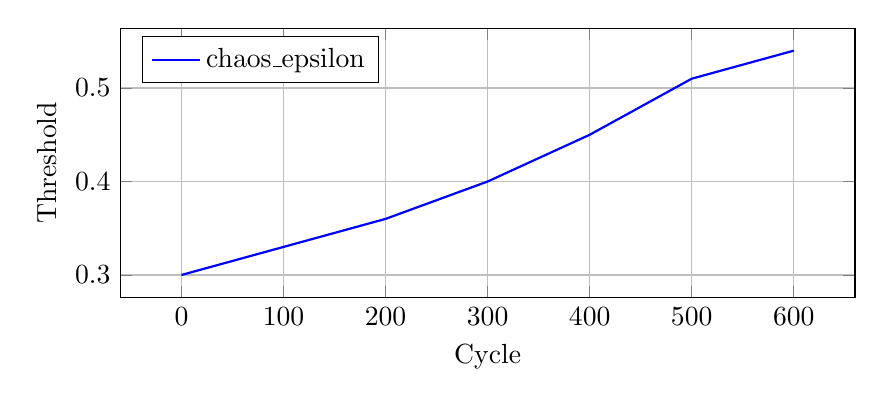
\begin{tikzpicture}
\begin{axis}[
    width=0.9\textwidth, height=5cm,
    xlabel={Cycle}, ylabel={Threshold},
    legend pos=north west,
    grid=major
]
\addplot[blue, thick] table {
    0 0.30
    100 0.33
    200 0.36
    300 0.40
    400 0.45
    500 0.51
    600 0.54
};
\addlegendentry{chaos\_epsilon}
\end{axis}
\end{tikzpicture}
\caption{Adaptation of the chaos epsilon threshold as system complexity increases linearly.}
\label{fig:adapt}
\end{figure}